


\subsection{Experiment 1}
\label{sec:4_6_Expresults}

The pool size $T$ is crucial, and this size should be analyzed carefully to avoid model duplication and degradation of the overall performance. The proposed ensemble was tested with 8 sizes $\in$ \{5, 10, 15, 20, 25, 30, 40, 50\} over 25 datasets with 50 runs per dataset (10 replicas · 5 folds) to obtain  10,000 record (8·25·50) of results. Each row from Table \ref{ens-size} corresponds to the average accuracy of 1250 records, which is used to identify a suitable ensemble size for the presentation of the final results.
From Table \ref{ens-size}, the highest average accuracy is obtained with $T=50$. GA is competitive with MFO over various ensemble sizes. The poorest values from the proposed SI algorithms are presented in \textit{italics} and correspond to WOA; however, they are better than those of other individual classifiers and combination methods. DT represents the average accuracy of the best individual of type DT. The same holds for all best individuals of types NB, Mlnom, KNN, and JRip. Figure \ref{Ens-plot} presents the superior performance of both (GA, MFO) over various combination methods. The most interesting result in this graph is that the proposed fusion method at a smaller ensemble size with $T=15$ (\textit{dotted horizontal line}) outperforms other combination methods for large ensemble sizes.



\begin{table}[t]
\centering
\caption{Ensemble size analysis for higher prediction accuracy over all 25 datasets. The best two values are shown in bold.}
\resizebox{\textwidth}{!}{
\begin{tabular}{c|c||c||ccccc||cccc||cccc}
  \hline
   & \multicolumn{2}{c}{Random Forest}    & \multicolumn{5}{c}{Individual Models} & \multicolumn{4}{c}{Cobmination Methods} & \multicolumn{4}{c}{Combination by GA and  SI}   \\ 
     \hline
 $T$ & RFCOM & RFSM & DT & NB & Mlnom & KNN & JRip & Maj & Belief & CW-NN & Stacking & GA & GWO & MFO & WOA \\ 
  \hline
\rule{0pt}{10pt} 5 & 78.26 & 77.41 & 72.10 & 70.87 & 74.95 & 72.82 & 71.07 & 78.01 & 78.43 & 77.73 & 77.51 &\textbf{78.99} & 78.96 & \textbf{78.97} & \textit{78.89}$\cdot$ \\ 
\rule{0pt}{10pt} 10 &\textbf{ 80.44} & 78.77 & 74.09 & 73.02 & 76.78 & 74.88 & 73.06 & 78.56 & 79.40 & 78.71 & 77.33 & \textbf{80.30} & 80.13 & 80.23 & \textit{80.03}$\cdot$ \\ 
\rule{0pt}{10pt} 15 &\textbf{ 81.32} & 79.39 & 75.18 & 74.29 & 77.70 & 75.77 & 73.83 & 79.48 & 79.88 & 78.99 & 77.15 & \textbf{80.91} & 80.72 & 80.88 & \textit{80.53}$\cdot$ \\ 
\rule{0pt}{10pt} 20 & \textbf{81.58} & 79.63 & 75.76 & 74.77 & 78.28 & 76.32 & 74.79 & 79.49 & 80.16 & 78.95 & 76.66 &\textbf{ 81.07} & 80.93 & 80.96 & \textit{80.63}$\cdot$ \\ 
\rule{0pt}{10pt} 25 & \textbf{82.05} & 79.79 & 76.19 & 75.16 & 78.67 & 76.74 & 75.14 & 79.86 & 80.32 & 78.94 & 76.28 & 81.16 & 81.15 & \textbf{81.17} & \textit{80.77}$\cdot$ \\ 
\rule{0pt}{10pt} 30 & \textbf{82.16} & 79.86 & 76.42 & 75.41 & 78.92 & 77.14 & 75.48 & 79.66 & 80.25 & 78.69 & 75.84 & 81.15 & 81.23 & \textbf{81.27} & \textit{80.74}$\cdot$ \\ 
\rule{0pt}{10pt} 40 & \textbf{82.51} & 79.98 & 76.86 & 76.00 & 79.17 & 77.47 & 75.98 & 79.83 & 80.34 & 78.56 & 75.40 & \textbf{81.22} & 81.18 & 81.21 & \textit{80.79}$\cdot$ \\ 
\rule{0pt}{10pt} 50 & \textbf{82.42} & 80.12 & 77.40 & 76.51 & 79.67 & 77.86 & 76.47 & 80.07 & 80.58 & 78.23 & 74.91 & 81.30 & 81.38 &\textbf{ 81.49} &\textit{81.07}$\cdot$ \\ 
   \hline
\end{tabular}
}
\label{ens-size}
\end{table}




\begin{figure*}[!ht]
\centering
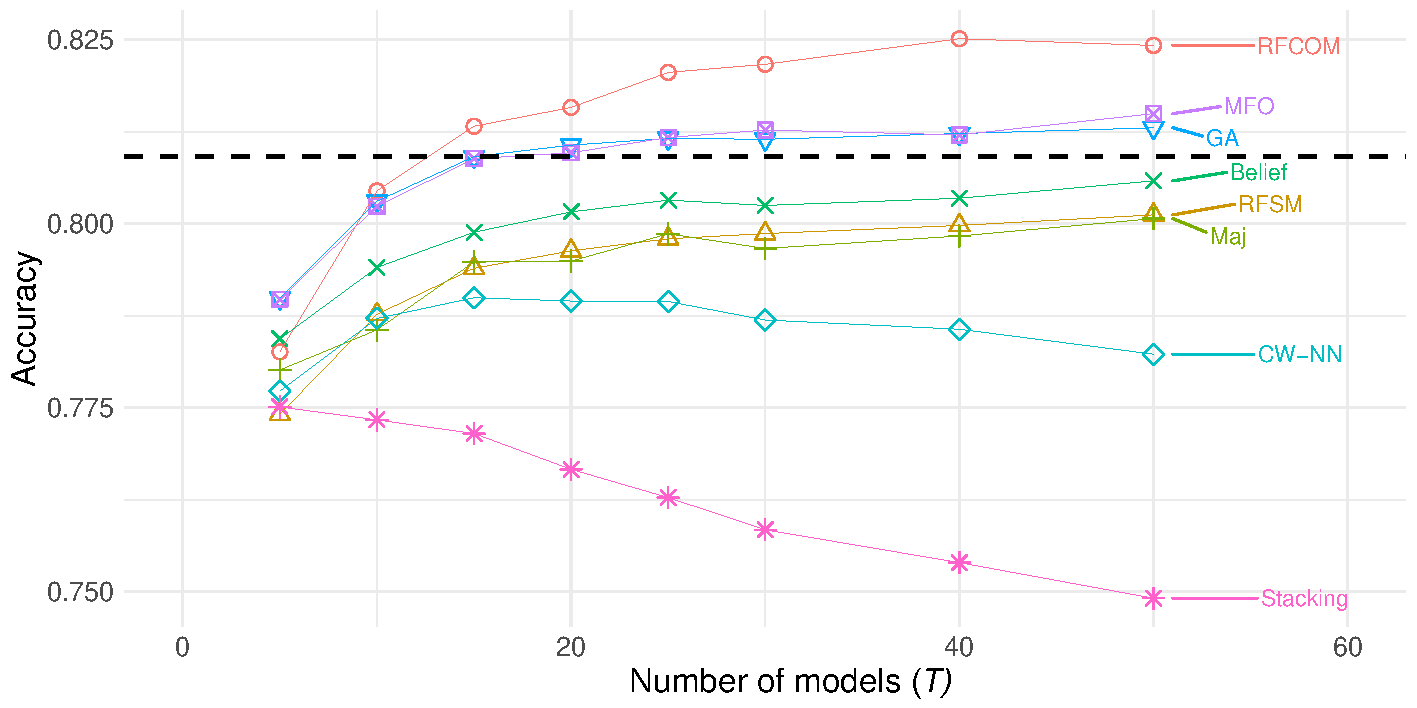
\includegraphics[width=.9\textwidth]{4_Taxonomy/figures/fig-Ens-plot.pdf}
\caption{Correlation between ensemble size and prediction accuracy that is averaged over all the datasets.}
\label{Ens-plot}
\end{figure*}




\subsection{Experiment 2} \label{comb.SI}
To present the final results, we selected an ensemble size of $T=50$. Hence, we have 10 models for each classifier type $\in$ \{DT, NB, Mlnom, KNN, JRip\}. Table  \ref{table-accuracy} presents the average accuracy on each dataset that is realized by RFCOM, RFSM, the best individual type, and various combination methods (Maj, Belief, CW-NN, Stacking). The results will be analyzed in terms of the research questions.  

\textbf{To answer} $\pmb{Q_1}$, we analyze the effect of data reduction. For that, the effect of AllKNN \cite{tomek1976} is analyzed via comparing the results that were obtained by both RFCOM and RFSM, in the presence of a realized reduction rate that results in fast ensemble learning. From Table \ref{table-accuracy}, RFSM realized only 4 improvements over RFCOM according to (\textit{$D_2$, $D_4$, $D_9$, $D_{17}$}). The highest improvement in accuracy over RFCOM reaches 3.47\% for \textit{$D_{17}$}. For \textit{$D_8$}, the reduction capacity (Red-Rate) is the highest, where the reduced training subset reaches 18.75\% on the complete training set without a large deviation in precision from the RFSM side. Furthermore, for \textit{$D_5$}, RFCOM outperforms RFSM with 1.85\%, but it uses the complete training set, while RFSM uses only 45\% as a training subset. Finally, the training set selection time (Tss-TM) is problem-dependent and differs according to the number of samples and the number of features. The slowest time is 220.59 seconds for \textit{$D_{21}$}, while the fastest selection time is 2.4 seconds for \textit{$D_8$}.


\afterpage{
\begin{landscape}
\begin{table}[!ht]
  \centering
\caption{Average accuracy for $T=50$. The best two values are in bold, while the best from GA and SI is in \textit{italic}.}
\label{table-accuracy}
\renewcommand{\arraystretch}{1.3}
\begin{adjustbox}{max width=1.4\textwidth}
\begin{tabular}{ll|cc||cc||ccccc||cccc||cccc}
  \hline
   &  & \multicolumn{2}{c}{AllKNN} & \multicolumn{2}{c}{Random Forest}    & \multicolumn{5}{c}{Individual Models} & \multicolumn{4}{c}{Combination Methods} & \multicolumn{4}{c}{Combination by GA and  SI}   \\
  \hline
 \#& Data & Red\_Rate & Tss\_TM & RFCOM & RFSM & DT & NB & \multicolumn{1}{c}{Mlnom} & KNN & JRip & Maj & Belief & CW-NN & Stacking & GA & GWO & MFO & WOA \\ 
  \hline
$D_1$ & Australian & 0.26 & 9.13& 86.97 & 86.13 & \textbf{87.29} & 86.01 & \textbf{87.22} & 86.67 & 86.45 & 85.97 & 86.16 & 83.48 & 83.58 & 86.23 & 86.04 & \textit{86.33}$\cdot$  & 86.13 \\ 
  $D_2$ & Balance & 0.28 & 6.45 & 84.18 & 85.73 & 71.76 & 73.62 & 73.60 & 72.21 & 72.13 & 82.06 & 82.29 & 83.76 & 86.21 &\textbf{86.31} & 86.23 & \textbf{\textit{86.50}}$\cdot$ & 86.10 \\ 
  $D_3$ & Biodegradation & 0.25 & 21.99 &\textbf{ 86.25} & 85.26 & 84.67 & 73.18 & \textbf{86.81}& 84.61 & 84.07 & 85.64 & 86.16 & 83.86 & 83.24 & 85.93 & \textit{86.08}$\cdot$  & 86.00 & 85.89 \\ 
  $D_4$ & Dermatology & 0.07 & 8.21& 97.07 & 97.13 & 95.95 & 94.45 & 95.81 & 95.90 & 90.42 & 97.46 & \textbf{97.52} & 92.96 & 87.35 & 97.46 & 97.46 & \textit{\textbf{97.49}}$\cdot$ & 97.13 \\ 
 $D_5$ & Diabetic & 0.55 & 13.42 & 67.10 & 65.88 & 66.78 & 63.66 & \textbf{73.12} & 65.65 & 67.48 & 66.25 & 67.28 & 67.55 & 67.74 & 68.08 & 68.88 & 68.53 & \textit{\textbf{68.93}}$\cdot$  \\ 
  $D_6$ & Dna & 0.36 & 199.93 & 94.80 & 93.50 & 88.86 & 82.17 & 87.74 & 73.55 & 87.47 & 94.10 & 94.84 & 92.96 & 93.94 & 95.04 & \textbf{95.06} & \textbf{\textit{95.13}}$\cdot$  & 94.78 \\ 
  $D_7$ & German & 0.44 & 14.71 & \textbf{76.31} & 72.18 & 73.67 & 74.38 &\textbf{ 75.10} & 72.52 & 73.31 & 71.50 & 71.26 & 70.03 & 70.06 & 73.17 &\textit{ 73.50}$\cdot$  & 73.47 & 72.68 \\ 
  $D_8$ & Hert-Beach & 0.81 & 2.43 & 33.26 & 31.49 & \textbf{38.36} & 36.76 & \textbf{38.40} & 37.64 & 37.35 & 31.51 & 31.49 & 28.85 & 29.83 & \textit{31.66}$\cdot$  & 31.14 & 31.62 & 30.58 \\ 
  $D_9$ & Heart-Statlog & 0.34& 6.53 & 81.33 & 81.37 & 83.04 & \textbf{84.11} & \textbf{85.00} & 83.00 & 83.15 & 82.96 & 83.04 & 77.15 & 79.07 & \textit{82.85}$\cdot$  & 82.41 & 82.48 & 81.37 \\ 
  $D_{10}$ & Ionosphere & 0.18 & 12.18 & \textbf{93.28} & 91.31 & 90.83 & 91.60 & 88.55 & 86.33 & 91.26 & 89.21 & 89.55 & 91.20 & \textbf{91.97} & 90.72 & 90.43 & 91.14 & \textit{91.60}$\cdot$  \\ 
 $D_{11}$ & Mf-fourier & 0.28 & 71.93 & \textbf{82.71} & 80.02 & 72.27 & 75.76 & 71.47 & 77.36 & 68.57 & 79.94 & 80.19 & 69.86 & 54.46 & 80.57 & \textbf{\textit{80.96}}$\cdot$  & 80.86 & 80.14 \\ 
  $D_{12}$ & Mf-karh & 0.07 & 62.94 & 95.46 & 94.86 & 78.49 & 91.61 & 89.37 & 93.01 & 76.44 & \textbf{96.01} & \textbf{96.07} & 89.04 & 65.35 &\textit{96.00}$\cdot$  & 95.87 & 95.88 & 95.44 \\ 
  $D_{13}$ & Mf-zernike & 0.26 & 51.83 & 77.08 & 75.60 & 67.32 & 73.42 & 78.77 & 80.02 & 64.82 & 80.62 & 80.26 & 76.62 & 57.38 & \textbf{80.83} & \textbf{\textit{81.02}}$\cdot$  & 80.75 & 80.30 \\ 
  $D_{14}$ & Mov-Libras & 0.32 & 13.19 & \textbf{81.14} & 64.23 & 57.25 & 57.32 & 67.68 & 63.89 & 45.39 & 66.21 & \textbf{69.08} & 59.42 & 29.56 & 67.74 &\textit{68.87}$\cdot$  & 68.66 & 67.21 \\ 
  $D_{15}$ & Newthyroid & 0.07 & 3.75 & 95.81 & 93.86 & 95.49 & \textbf{98.05 }& \textbf{97.30} & 95.86 & 95.02 & 95.12 & 95.40 & 93.44 & 95.44 & 95.67 & 95.44 & \textit{95.91}$\cdot$ & 94.98 \\ 
  $D_{16}$ & Ringnorm & 0.32 & 125.09 & 94.81 & 93.03 & 85.81 & 93.61 & 71.17 & 68.19 & 87.06 & 86.01 & 91.73 & 96.86 & 96.66 & 97.06 & \textbf{\textit{97.23}}$\cdot$  & \textbf{97.18} & 96.93 \\ 
  $D_{17}$ & Sa-Heart & 0.49 & 5.19 & 67.97 & 70.32 & 73.20 & 73.40 & \textbf{74.57} & 72.81 &\textbf{74.18} & 71.10 & 71.36 & 66.49 & 66.97 & 71.02 & 71.13 & \textit{71.62}$\cdot$  & 71.02 \\ 
  $D_{18}$ & Sonar & 0.22 & 6.43 & \textbf{81.98} & 78.36 & 78.90 & 74.72 & 79.67 & \textbf{83.13} & 79.52 & 78.18 & 78.62 & 75.82 & 77.92 & 78.09 & 78.58 & 78.72 & \textit{78.76}$\cdot$  \\ 
  $D_{19}$ & Tae & 0.70 & 2.81 & \textbf{62.96} & 49.61 & 54.89 & \textbf{55.05} & 54.03 & 54.13 & 53.81 & 48.08 & 47.96 & 51.32 & 50.38 & 49.94 & 49.29 &\textit{50.34}$\cdot$ & 49.72 \\ 
  $D_{20}$ & Thyroid-dis & 0.48 & 48.04 & \textbf{70.79} & 69.84 & 68.32 & 35.40 & \textbf{69.96} & 67.60 & 68.18 & 69.58 & 69.35 & 65.46 & 63.93 & \textit{69.95}$\cdot$& 69.53 & 69.53 & 69.63 \\ 
  $D_{21}$ & Twonorm & 0.08 & 220.59 & 96.78 & 96.66 & 84.91 & 94.75 & 94.61 & 91.41 & 88.58 & \textbf{97.49} & \textbf{97.51} & 96.50 & 96.59 &\textit{97.38}$\cdot$ & 97.31 & 97.32 & 97.35 \\ 
  $D_{22}$ & Vehicle & 0.41 & 12.78 & \textbf{74.89} & 70.47 & 68.18 & 55.82 & 72.31 & 67.19 & 66.18 & 68.77 & 69.03 & 69.22 & 69.34 & 71.40 &\textbf{\textit{ 73.16}}$\cdot$ & 72.64 & 71.31 \\ 
  $D_{23}$ & Waveform & 0.32 & 78.21 & 84.76 & 84.46 & 76.99 & 81.68 & 84.02 & 79.14 & 78.23 & 84.40 & 84.86 & 82.69 & 83.12 & \textbf{\textit{85.78}}$\cdot$ & 85.39 & \textbf{85.66} & 85.38 \\ 
  $D_{24}$ & Wdbc & 0.07 & 11.70 & 95.71 & 95.08 & 95.80 & 95.36 & \textbf{98.07} &\textbf{ 97.37} & 95.94 & 96.19 & 96.19 & 95.68 & 96.66 & 96.40 & 96.29 & 96.38 & \textit{96.50}$\cdot$ \\ 
  $D_{25}$ & Wisconsin & 0.06 & 9.49 & 97.09 & 96.59 & 95.93 & 96.97 & \textbf{97.51} & 97.22 & 96.85 & \textbf{97.33} & 97.32 & 95.43 & 96.03 & \textit{97.25}$\cdot$& 97.12 & 97.20 & 96.93 \\ 
\hline
 & \textbf{AR-Friedman} &  &  & 5.44 & 9.5 & 9.42 & 9.66 & 5.92 & 8.92 & 10.04 & 8.48 & 6.94 & 11.64 & 10.86 & \textbf{5.4} & 5.94 & \textbf{4.84} & 7 \\ 
\hline
\end{tabular}
\end{adjustbox}
\end{table}
\end{landscape}
}







\textbf{To answer} $\pmb{Q_2}$, we analyze the effect of SI. The prediction accuracy of the proposed ensemble is compared with those of individual classifiers, various combination methods, and RFSM. The comparison includes the last 14 columns from Table \ref{table-accuracy} since all use only the reduced data. The best prediction accuracy for each dataset is highlighted in bold, while the value in italics represents the best from the proposed combination. The results demonstrate the performance of Mlnom as an individual classifier and Belief as a combination method. The average accuracy for each base classifier is based on the selection of the best classifier from the corresponding type; however, the degradation in the performance of those individuals is too large compared to the performances of the proposed strategies. For example, the accuracy of Mlnom reaches 71.17\% according to \textit{$D_{16}$}, while the proposed fusion realizes 97.23\%. For \textit{$D_2$}, Mlnom classifies 73.6\% correctly, while 86.5\% is the highest prediction accuracy that is realized by SI. The highest prediction by Mlnom compared with SI has been recorded as 6.7\% for \textit{$D_8$}.  
Thus, the deviation in the prediction accuracy level is highly significant. For the combination methods, the Belief function realizes 91.7\% accuracy for \textit{$D_{16}$}, while the highest prediction accuracy is 97.2\% by SI. At least one SI algorithm outperforms RFSM for all 25 datasets, and the highest percentages of improvement are 7.23\% and 4.5\% over RFSM for \textit{$D_{14}$} and \textit{$D_{16}$}, respectively.


 
 
 It is interesting to connect this part with the previous section to prove how the proposed fusion mechanisms outperform learning from nonreduced data in terms of prediction accuracy. Comparing with RFCOM, the proposed fusion mechanism using meta-heuristics outperforms RFCOM on 14 datasets \{$D_2$, $D_4$, $D_5$, $D_6$, $D_9$, $D_{12}$, $D_{13}$, $D_{15}$, $D_{16}$, $D_{17}$, $D_{21}$, $D_{23}$, $D_{24}$, $D_{25}$
 \} with maximum improvement percentages of  5.38\% and 5.11\% on \textit{$D_{17}$ and $D_{13}$}, respectively. Figure \ref{histogramplots} presents the ordered histograms of all combination methods (left to right) for comparisons against RFCOM.    
 \vspace*{.4cm}
 
 \begin{figure*}[!ht]
\begin{center}
  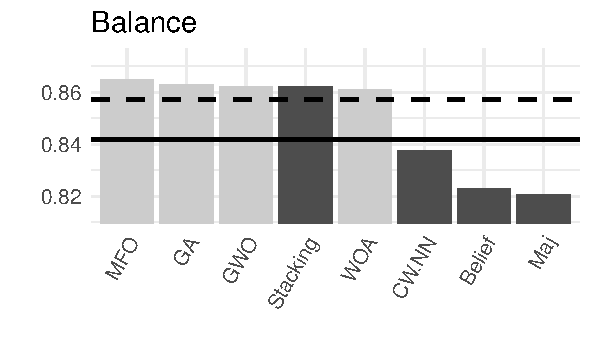
\includegraphics[width=.3\textwidth]{4_Taxonomy/figures/Balance.pdf}
  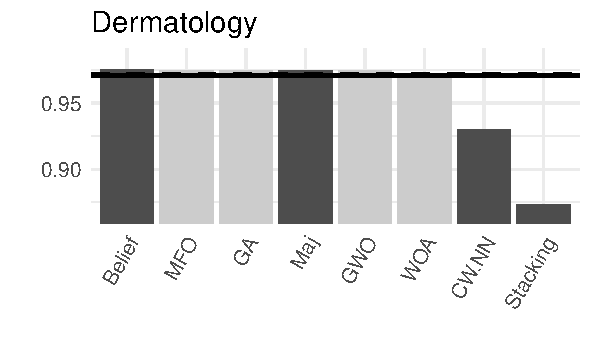
\includegraphics[width=.3\textwidth]{4_Taxonomy/figures/Dermatology.pdf}
  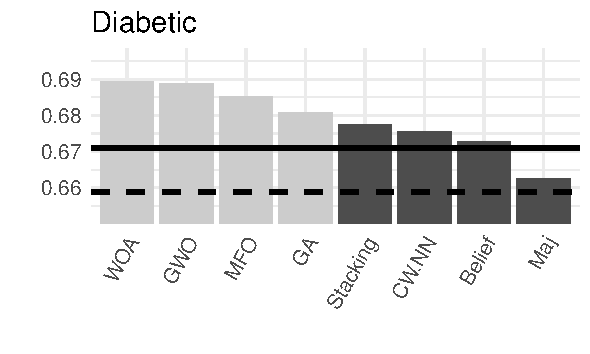
\includegraphics[width=.3\textwidth]{4_Taxonomy/figures/Diabetic.pdf}\\
  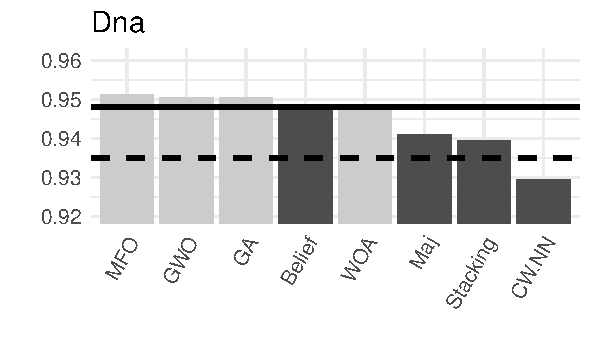
\includegraphics[width=.3\textwidth]{4_Taxonomy/figures/Dna.pdf}
  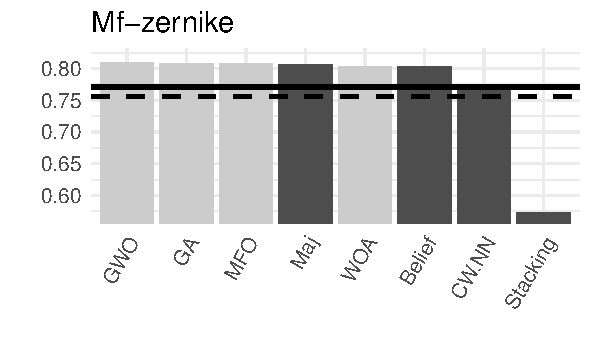
\includegraphics[width=.3\textwidth]{4_Taxonomy/figures/Mf-zernike.pdf}
  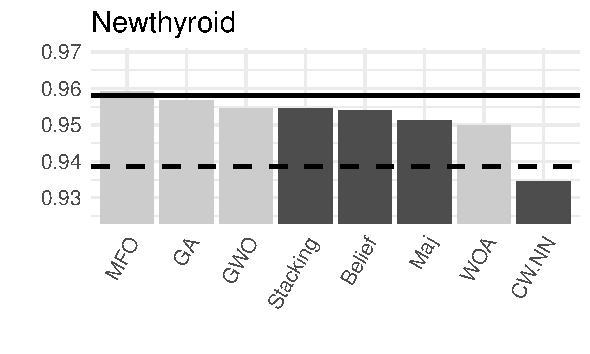
\includegraphics[width=.3\textwidth]{4_Taxonomy/figures/Newthyroid.pdf}\\
 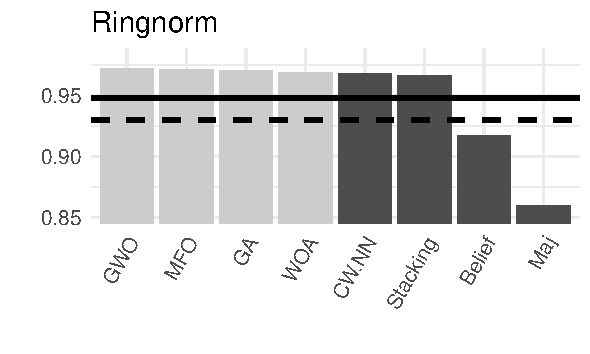
\includegraphics[width=.3\textwidth]{4_Taxonomy/figures/Ringnorm.pdf}
 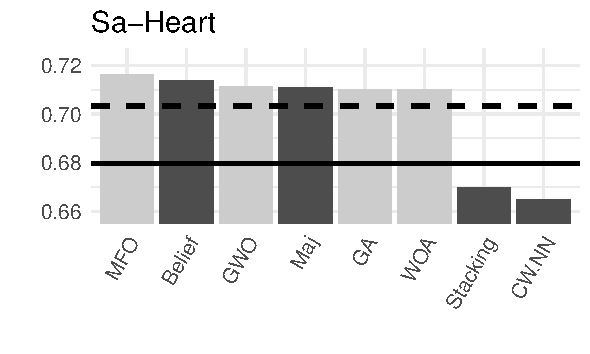
\includegraphics[width=.3\textwidth]{4_Taxonomy/figures/Sa-Heart.pdf}
  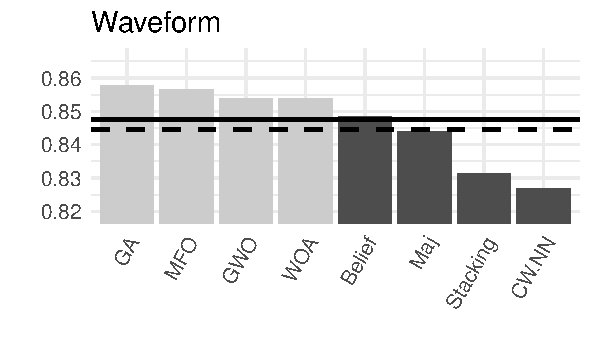
\includegraphics[width=.3\textwidth]{4_Taxonomy/figures/Waveform.pdf}

\end{center}
\caption{Comparing SI combination strategies against RFCOM (\protect\RFCOM) and RFSM (\protect\RFSM). Dark gray columns denote combination methods, while light gray columns denote SI strategies.}
\label{histogramplots}
\end{figure*}

 
 
 
 \subsection{Statistical Analysis of the Results} \label{statistical}
To compare the results, the null hypothesis of no improvement over the standard algorithms will be analyzed.  Two nonparametric statistical tests, namely, the Friedman test \cite{friedman1937} for multiple comparisons and the Wilcoxon signed ranks test \cite{wilcoxon1945} for pairwise comparisons, will be conducted. The average rank of the Friedman test \textit{(AR-Friedman)} is presented in the last row of Table \ref{table-accuracy}, with the best ranks scored sequentially as MFO, GA, RFCOM, Mlnom, and GWO. The Friedman statistic that was distributed according to the chi-square distribution with 14 degrees of freedom is 84.603, and the computed p-value is smaller than 0.01\%. 


Next, the Wilcoxon test \cite{wilcoxon1945} aims at detecting significant differences between the two sample means. From Table \ref{ch4:wilcoxontable}, none of the standard combination methods (Maj, Belief, Stacking, and CW-NN) outperforms RFSM, while our proposed combination methods (GA, GWO, MFO, and WOA) all significantly outperform RFSM by 95\%. Moreover, the proposed fusion methods are at the same level of competence as RFCOM. Further, Mlnom cannot outperform RFSM, Maj, or Belief which extends the superior performance of our proposed methods.
\vspace*{.3cm}

\begin{table*}[!ht]
\centering\scriptsize
\caption{Summary of the Wilcoxon test. \cmark = the method in the row improves the method of the column. \textopenbullet = the method in the column improves the method of the row. Upper diagonal of level significance $\alpha=0.9$, lower diagonal level of significance $\alpha=0.95$}
\resizebox{\textwidth}{!}{\begin{tabular}{
|l|c|c|c|c|c|c|c|c|c|c|c|c|c|c|c|}
\hline
&(1) &(2) &(3) &(4) &(5) &(6) &(7) &(8) &(9) &(10) &(11) &(12) &(13) &(14) &(15) \\
\hline
RFCOM (1)& -& \cmark & \cmark & \cmark &  & \cmark & \cmark & \cmark & \cmark & \cmark & \cmark &  &  &  &  \\
\hline
RFSM (2)& \textopenbullet & -& \cmark & \cmark &  &  & \cmark &  &  & \cmark & \cmark & \textopenbullet & \textopenbullet & \textopenbullet & \textopenbullet \\
\hline
DT (3)& \textopenbullet &  & -&  & \textopenbullet &  &  &  & \textopenbullet &  &  & \textopenbullet & \textopenbullet & \textopenbullet & \textopenbullet \\
\hline
NB (4)& \textopenbullet &  &  & -& \textopenbullet &  &  & \textopenbullet & \textopenbullet &  &  & \textopenbullet & \textopenbullet & \textopenbullet & \textopenbullet \\
\hline
Mlnom (5)&  &  & \cmark & \cmark & -& \cmark & \cmark &  &  & \cmark & \cmark &  &  &  &  \\
\hline
KNN (6)& \textopenbullet &  &  &  & \textopenbullet & -&  & \textopenbullet & \textopenbullet &  &  & \textopenbullet & \textopenbullet & \textopenbullet & \textopenbullet \\
\hline
JRip (7)& \textopenbullet & \textopenbullet &  &  & \textopenbullet &  & -& \textopenbullet & \textopenbullet &  &  & \textopenbullet & \textopenbullet & \textopenbullet & \textopenbullet \\
\hline
Maj (8)& \textopenbullet &  &  & \cmark &  &  &  & -& \textopenbullet & \cmark & \cmark & \textopenbullet & \textopenbullet & \textopenbullet & \textopenbullet \\
\hline
Belief (9)&  &  & \cmark & \cmark &  &  & \cmark & \cmark & -& \cmark & \cmark & \textopenbullet & \textopenbullet & \textopenbullet &  \\
\hline
CW-NN (10)& \textopenbullet & \textopenbullet &  &  & \textopenbullet &  &  & \textopenbullet & \textopenbullet & -&  & \textopenbullet & \textopenbullet & \textopenbullet & \textopenbullet \\
\hline
Stacking (11)& \textopenbullet & \textopenbullet &  &  & \textopenbullet &  &  & \textopenbullet & \textopenbullet &  & -& \textopenbullet & \textopenbullet & \textopenbullet & \textopenbullet \\
\hline
GA (12)&  & \cmark & \cmark & \cmark &  & \cmark & \cmark & \cmark & \cmark & \cmark & \cmark & -&  & \textopenbullet & \cmark \\
\hline
GWO (13)&  & \cmark & \cmark & \cmark &  & \cmark & \cmark & \cmark &  & \cmark & \cmark &  & -&  & \cmark \\
\hline
MFO (14)&  & \cmark & \cmark & \cmark &  & \cmark & \cmark & \cmark & \cmark & \cmark & \cmark & \cmark &  & -& \cmark \\
\hline
WOA (15)&  & \cmark & \cmark & \cmark &  &  & \cmark & \cmark &  & \cmark & \cmark & \textopenbullet & \textopenbullet & \textopenbullet & -\\
\hline

\end{tabular}}
\label{ch4:wilcoxontable}
\end{table*}



After statistical analysis and according to the average rank of the Friedman test, we selected \{MFO, GA, GWO, Mlnom, Belief, RFSM, RFCOM\} and analyzed the distribution of their prediction accuracy levels. Figure \ref{consprediction} presents the range of the prediction accuracy around the median and how the proposed fusion strategies realize robust and stable prediction for \{\textit{D$_2$, D$_4$, D$_6$, D$_{13}$, D$_{16}$, D$_{23}$\}}.    



 \begin{figure*}[!ht]
\begin{center}
  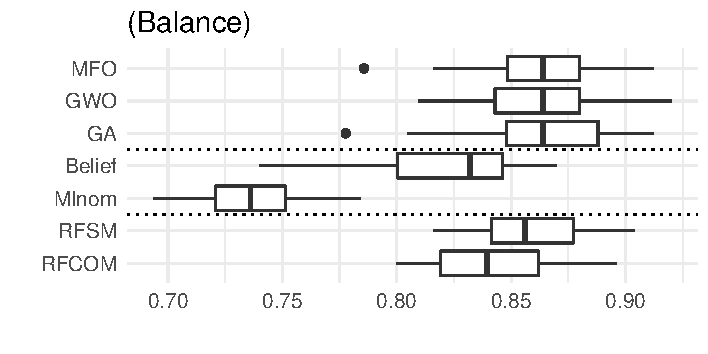
\includegraphics[width=.49\textwidth]{4_Taxonomy/figures/boxplot-Balance.pdf}
  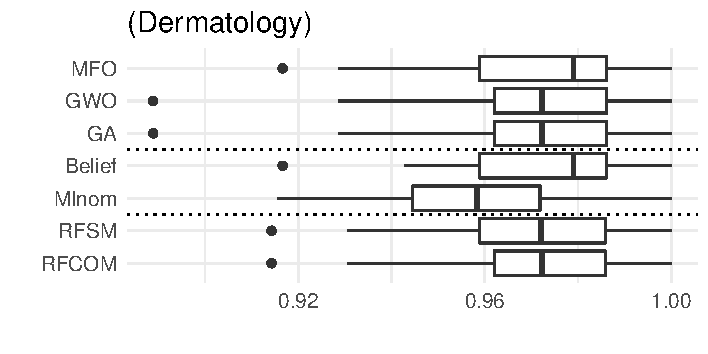
\includegraphics[width=.49\textwidth]{4_Taxonomy/figures/boxplot-Dermatology.pdf} \\
  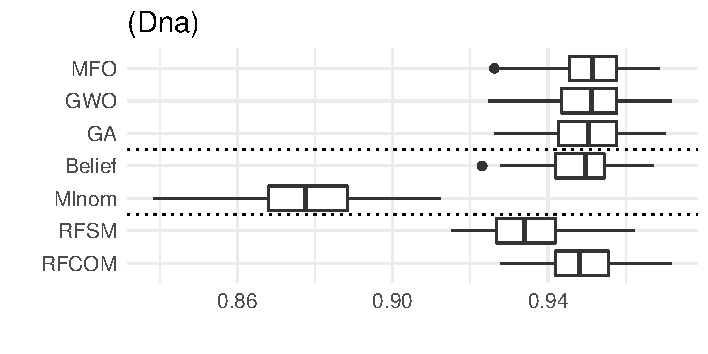
\includegraphics[width=.49\textwidth]{4_Taxonomy/figures/boxplot-Dna.pdf}
  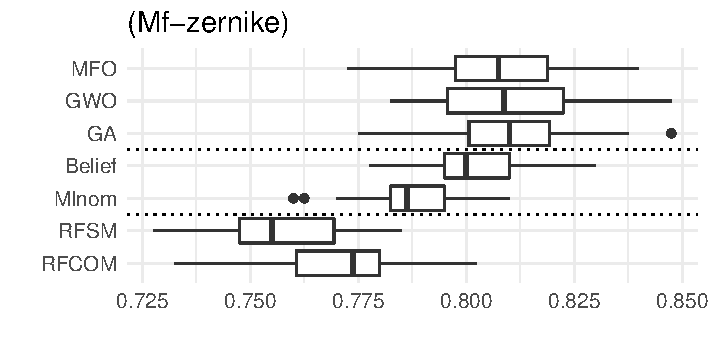
\includegraphics[width=.49\textwidth]{4_Taxonomy/figures/boxplot-Mf-zernike.pdf}\\
  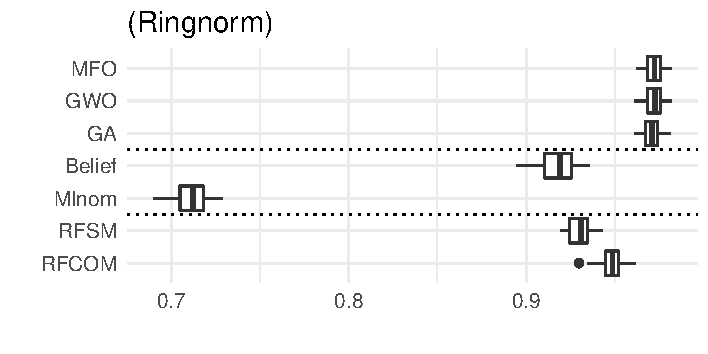
\includegraphics[width=.49\textwidth]{4_Taxonomy/figures/boxplot-Ringnorm.pdf}
  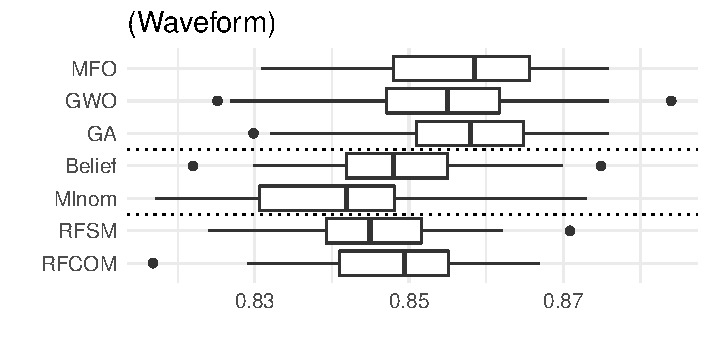
\includegraphics[width=.49\textwidth]{4_Taxonomy/figures/boxplot-Waveform.pdf}
\end{center}
\caption{Distribution of the prediction accuracy.}
\label{consprediction}
\end{figure*}

\subsection{Exploration of the Research Questions} \label{ch4:explorationofres}

In this part, we determine whether the research questions of the first objective are answered or not. 

\textit{\textbf{($\pmb{Q_1}$)}  The impact of reduced and consistent data on the performance of the ensemble learning} can be identified, but it depends mainly on the building schema of the ensemble.

\begin{enumerate}[nosep]

    \item [--] Random forest: RFSM outperformed RFCOM on only 4 datasets, as presented in the first part of Section \ref{comb.SI}.
    \item[--] Proposed MCS in Section \ref{proposed.mcs}: The simple majority voting (Maj) of the proposed MCS outperformed RFCOM on 8 datasets (D$_4$, D$_9$, D$_{12}$, D$_{13}$, D$_{17}$, D$_{21}$, D$_{24}$, and D$_{25}$), while the class degree (Belief) outperformed RFCOM on 11 datasets (D$_4$, D$_5$, D$_6$, D$_9$, D$_{12}$, D$_{13}$, D$_{17}$, D$_{21}$, D$_{23}$, D$_{24}$, and D$_{25}$).
    \item[--] The conclusion, IS proved its effectiveness to reduce the training data-size of 17 datasets by more than 25\%. AllKNN, as IS technique, did not prove its capability to capture the integrity from the whole data. The proposed MCS could compensate the error of IS method. 
\end{enumerate} 

\textit{\textbf{($\pmb{Q_2}$)}  The search capability of swarm intelligence to enhance the combination of classifiers} has been evaluated and discussed in the last part of Section \ref{comb.SI} with SI outperforming RFCOM on 14 datasets. The conclusion that SI algorithms are so effective to optimize the classifiers' combination function.  


